%=====================
%  EXPERIMENTS
%=====================

We now applied the idea of Support Vector Machines to classifying handwritten digits from the MNIST dataset\cite{mnist}. The MNIST database consists of $70,000$ correctly labeled images of handwritten digits, that are size-normalized and centered. $60,000$ of them belong to the training set i.e., these images are used in finding the optimal hyperplane. The remaining $10,000$ belong to the testing set i.e., we test the accuracy of our hyperplanes with these images. All of them are $28\times28$ pixel images of a handwritten single digit. Figure \ref{fig:mnist} shows some sample images from the dataset.

\begin{figure}[!tb]
	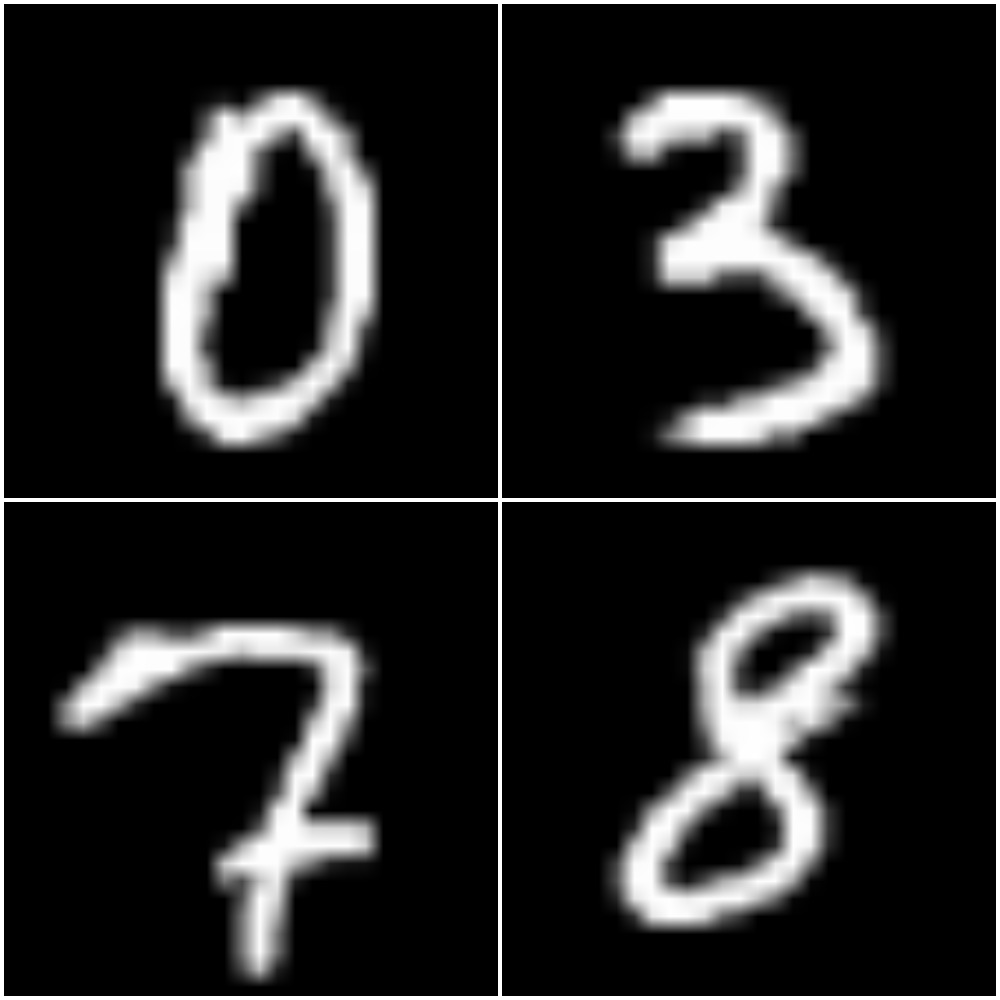
\includegraphics[width=4cm, height=4cm]{mnist_sample}
	\centering
	\caption{Sample images from MNIST dataset}
	\label{fig:mnist}
\end{figure}

Our classification problem is that of learning to recognize the correct digit. With classifying digits, we have $10$ different classes i.e., $\{0, 1, 2, 3, 4, 5, 6, 7, 8, 9\}$. Since this is a multi-class classification problem (there are more than $2$ classes), we employed the one-versus-rest classification technique. In this technique, we construct $10$ different hyperplanes - each hyperplane distinguishes the input image between one class and the rest. For example, one such hyperplane would classify the input image as either $0$, or not. Another hyperplane would classify the input image as either $3$, or not. Thus, we constructed $10$ different hyperplanes. Note that we need $10$, and not $9$, hyperplanes to account for the possibility that the image we are classifying might not be any of the $10$ digits. Given an image, we then looped through each of $10$ hyperplanes and check if the image belongs to that class. A drawback with this method is that we also run into the possibility of the same image being assigned to two different classes. When that happened, we chose the hyperplane that gives a higher output value for the image.

Before actually finding the optimal hyperplanes, let us introduce some old notation to our new data. Let the number of training images be $m$. Let $\vec{X}\in\mathbb{R}^{m}$, be the vector of all the images from the training set. Let us denote each element of $\vec{X}$ as $\vec{x_i}$, which is, in turn, a single image. Usually images are matrices with pixel values as entries for the matrix. Here, we unrolled the $2$-D matrix into a one dimensional vector. Let the length of the unrolled vector be $n$. Therefore, $\vec{x_i}\in\mathbb{R}^{n}$. Hence, it might make sense to think of $\vec{X}$ as a matrix, $X\in\mathbb{R}^{m \times n}$. Thus, the pixel values of the image become features in our input feature space. Since we are working with gray-scale images, we do not have to worry about RGB channels. In our case, $m = 60,000$, and $n = 28\times28 = 784$.

Our ${y_i}$ associated with each of the $\vec{x_i}$ depends on the hyperplane we are constructing. Assume we are constructing the $k^{th}$ hyperplane i.e., the hyperplane that classifies the image as either digit $k$, or not digit $k$. Then $y_i = 1$ if image $\vec{x_i}$ represents digit $k$, and $y_i = -1$ otherwise. These values follow from our mathematical formulation in Section \textbf{\ref{section:math}}. Let us define the normal to this hyperplane as $\vec{w}^{(k)}$. Since our $y_i$ depends on the value $k$, let us re-define our notation as $y^{(k)}_i$, where
\begin{equation*}
    y^{(k)}_i= 
\begin{cases}
\begin{aligned}
 1,& \text{ if } x_i \text{ represents } k\\
-1,              & \text{ otherwise}
\end{aligned}
\end{cases}
\end{equation*}

With this modified notation, we now trained the support vector machine and obtain our $10$ hyperplanes. As discussed previously, for predicting the digit on an image, we can use equation (\ref{eq:ovr-decision}) that uses our new notation.
\begin{equation}
	f^{(k)}(x_i) = \vec{w}^{(k)}\cdot\vec{x_i} + b \label{eq:ovr-decision}
\end{equation}
If $f^{(k)}(x_i) \geq 0$, then $\vec{x_i}$ represents $k$, and it does not represent $k$ otherwise. If, using this method, we find that $\vec{x_i}$ represents multiple $k_j$, then we choose a $k_a$ such that
\begin{equation*}
	f^{(k_a)}(x_i) = \max_{j} f^{(k_j)}(x_i)  \label{eq:ovr-conflict}
\end{equation*}

Finally, to make computation simpler, we set the intercept as the origin i.e., $b = 0$. Since the optimization problem is beyond the scope of this project, we used \texttt{sklearn}\cite{scikit-learn} library to help us with the optimization process.